% DOCUMENT
\documentclass[oneside,14pt,a4paper]{extreport}

% LANGUAGE
\usepackage[T2A]{fontenc}
\usepackage[utf8]{inputenc}
\usepackage[english, ukrainian]{babel}

% VARIABLES
\newcommand \labno    {2}
\newcommand \course   {Візуалізація даних}
\newcommand \group    {310}
\newcommand \lecturer {Бойко Наталія Іванівна}
\newcommand \theme    {Аналіз даних	та статистичне виведення}
\newcommand \purpose  {[Мета звіту]}

% PACKAGES
\usepackage{amssymb}
\usepackage{amsmath}
\usepackage{multirow}
\usepackage{pgfplots}

% GEOMETRY
\usepackage{geometry}
\geometry{left   = 2.5cm}
\geometry{right  = 1cm}
\geometry{top    = 2cm}
\geometry{bottom = 2cm}
\renewcommand {\baselinestretch} {1.5}
\setlength\parindent{1cm}

% IMAGES
\usepackage{graphicx}
\usepackage{indentfirst}
\graphicspath{ {./imgs/} }

% FOOTER
\usepackage{scrpage2}
\ifoot[]{}
\cfoot[]{}
\ofoot[\pagemark]{\pagemark}
\pagestyle{scrplain}

% CHAPTERS

\newcommand\Section[1]{
 \refstepcounter{section}
 \section*{
  \arabic{section}. #1}
}

\newcommand\Subsection[1]{
 \refstepcounter{subsection}
 \section*{
  \arabic{section}.\arabic{subsection}. #1}
}

\sloppy
\begin{document}
\begin{titlepage}

\centering
 \textbf{
  МІНІСТЕРСТВО ОСВІТИ І НАУКИ УКРАЇНИ \\
  НАЦІОНАЛЬНИЙ УНІВЕРСИТЕТ \flqq{}ЛЬВІВСЬКА ПОЛІТЕХНІКА\frqq{}
 }

\vspace{1.5cm}
 \textbf{
  Інститут комп'ютерних наук та інформаційних технологій \\
  Кафедра систем штучного інтелекту
}

\vspace*{\fill}

  {\textbf{Лабораторна робота №\labno}
   \par}
  {З курсу \flqq\course\frqq \par}

\vspace{1cm} \theme

\raggedleft\vfill

 {\textbf{Виконав:} \par}
 {ст. гр. КН-\group \par}
 {Бікєєв Андрій \par}

\vspace{1cm}

 {\textbf{Викладач:} \par}
 {\lecturer \par}

\vspace{1cm}

\centering {Львів -- \the\year \par}

\end{titlepage}

\Section{Хід роботи}

\Subsection{Імпортування бібліотек і даних}
\small
\begin{verbatim}
import pandas as pd
import matplotlib.pyplot as plt 
import numpy as np
import statsmodels.api as sm

df = pd.read_csv("filmdeathcounts.csv")
\end{verbatim}

Ці бібліотеки допоможут в візуалізації даних. та побудові графіків. Дані імпортуються з файлу filmdeathcounts.csv.

\Subsection{Додавання поля body\_per\_min, з відношення всіх вбитих у фільмі до довжини фільму у хвилинах}
\small
\begin{verbatim}
data["body_per_min"] = data["Body_Count"] / data["Length_Minutes"]
\end{verbatim}

\Subsection{Побудова гістограми для кількості персонажів, які загинули}
\small
\begin{verbatim}
data['Body_Count'].plot(kind="hist", edgecolor="black", color="cyan", bins=40)
plt.xlabel("Body_Count")
plt.show()
\end{verbatim}

\begin{figure}[!htb]
 \centering
 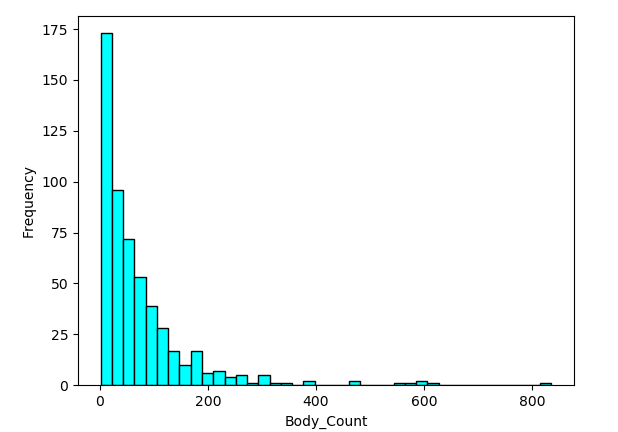
\includegraphics[scale=1.0]{graph_1}
 \caption{Гістограма "Загинувші персонажі"} 
\end{figure}

На цьому графіку можна побачити 5 розподілів, а також "глобальну" моду усього графіка(а також моду розподілу $0-200$), вона дорівнює нулю. Отже, найбільше фільмів у виборці - це таких, в яких ніхто не загинув.
Також ми бачимо, що кількість фільмів обернено пропорційна кількості загинувших персонажів, а отже цей графік можливо апроксимувати деякою функцією $y = (a/(bx + d)) + c$, де y - це кількість фільмів, а x - кількість загинувших персонажів, а a, b, c, d - деякі коефіцієнти для апроксимізації.

\clearpage
\Subsection{Топ 10 фільмів в яких загинуло більше всього персонажів}
\small
\begin{verbatim}
print(data.sort_values(by=['Body_Count'], ascending=False).head(10))
print(data.sort_values(by=['body_per_min'], ascending=False).head(10))
\end{verbatim}

\begin{figure}[!ht]
 \centering
 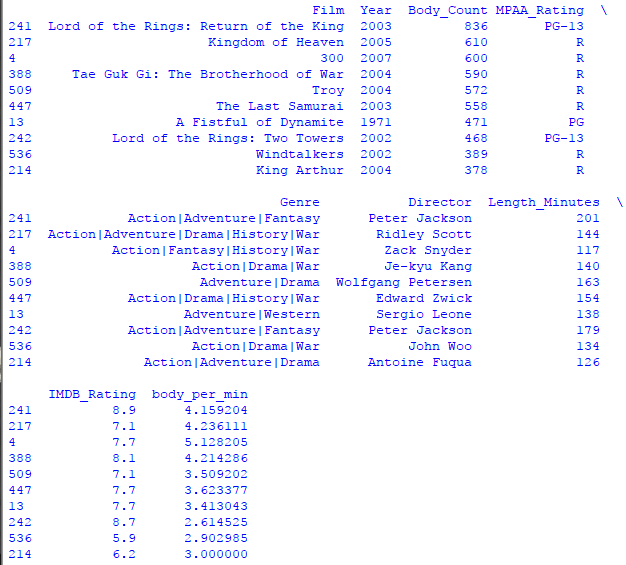
\includegraphics[scale=1.0]{result_1}
 \caption{Топ 10 за кількістью загинувших персонажів} 
\end{figure}
\clearpage

\begin{figure}[!ht]
 \centering
 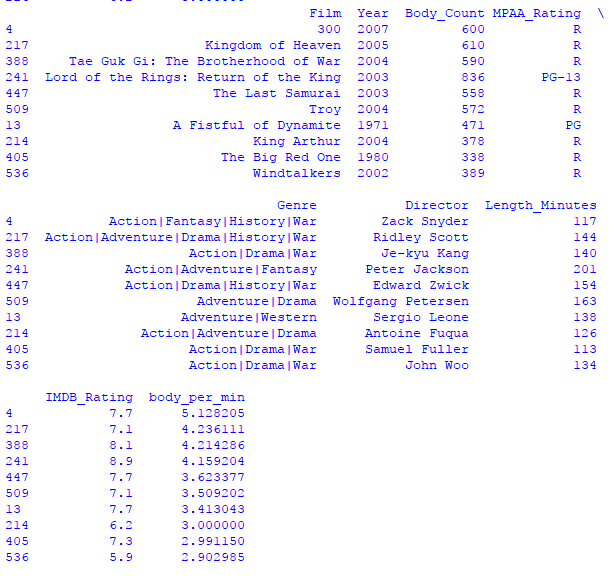
\includegraphics[scale=1.0]{result_2}
 \caption{Топ 10 за кількістью загинувших персонажів у відношенні до довжини фільму}
 \label{Топ10пермінут}
\end{figure}

З цих таблиць, можемо помітити, що за обома критеріями "найжорстокішими" фільмами є фільми жанру Action, Adventure, History, і War.
З таблиці два(на малюнку. \ref{Топ10пермынут})

\Subsection{Побудова гістограми для IMDb рейтингу}
\small
\begin{verbatim}
data['IMDB_Rating'].plot(kind="hist", edgecolor="black", color="cyan", bins=20)
plt.xlabel("IMDB_Rating")
plt.show()
\end{verbatim}

\begin{figure}[!ht]
 \centering
 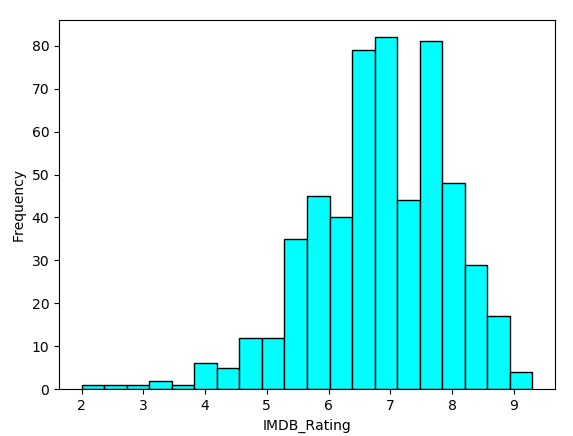
\includegraphics[scale=1.0]{graph_2}
 \caption{Гістограма "IMDb рейтинг"} 
\end{figure}

З цієї діаграми можна побачити, що більшість фільмів мають рейтинг більший ніж 5, що є дивним, адже цю оцінку ми вважаємо за "середню". "Глобальною" модою цієї діаграми є $~7$, у той час, як середнє значення прибзлино $~7.5$, що означає. що розподіл не є нормальним.

\Subsection{Симуляція гістограми IMDb рейтингу}
Порахуємо середнє значення, та середньоквадратичне відхилення для цієї вибірки, і побудуємо нормальну діаграму з такими значеннями.
\small
\begin{verbatim}
imdb_mean = data['IMDB_Rating'].mean()
imdb_sd = data['IMDB_Rating'].std()

data['imdb_simulation'] = np.random.normal(imdb_mean, imdb_sd, len(data.index))
data['imdb_simulation'].plot(kind="hist", edgecolor="black", color="cyan", bins=40)
plt.xlabel("imdb_simulation")
plt.show()
\end{verbatim}

\begin{figure}[!ht]
 \centering
 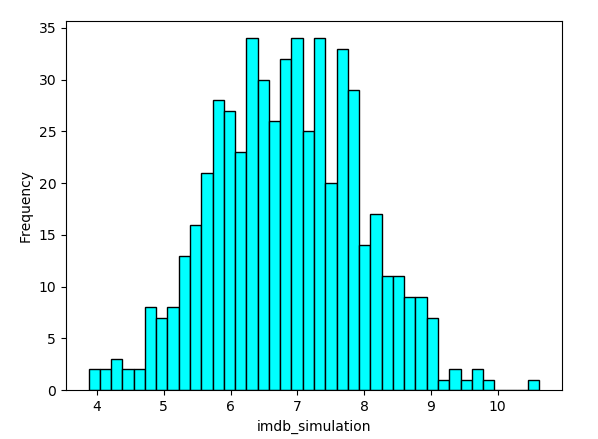
\includegraphics[scale=1.0]{graph_3}
 \caption{Гістограма "Симуляція IMDb рейтингу"} 
\end{figure}
\clearpage
\Subsection{Перевірка нормальності розподілу}

Для перевірки нормальності розподілу симуляції, а також даної вибірки побудуємо Q-Q діаграму.
\small
\begin{verbatim}
sm.qqplot(data['imdb_simulation'])
plt.xlabel("imdb_simulation")
plt.show()
\end{verbatim}
\clearpage

\begin{figure}[!ht]
 \centering
 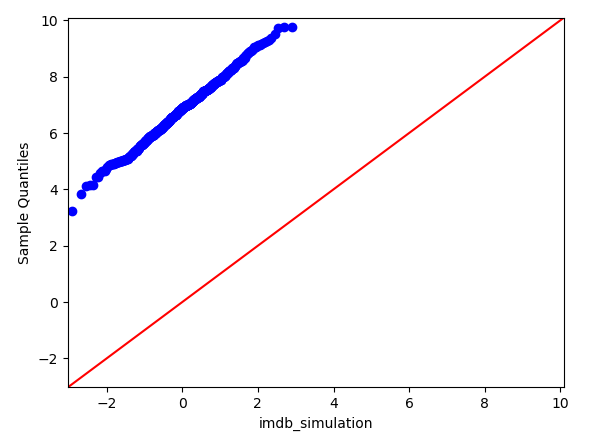
\includegraphics[scale=1.0]{graph_4}
 \caption{Q-Q діаграмма для "Симуляції IMDb рейтингу"} 
\end{figure}

Лінійність графіку симуляції показує, що ця вибірка є з нормальни розподілом.
\clearpage

\small
\begin{verbatim}
sm.qqplot(data['IMDB_Rating'])
plt.xlabel("IMDB_Rating")
plt.show()
\end{verbatim}

\begin{figure}[!ht]
 \centering
 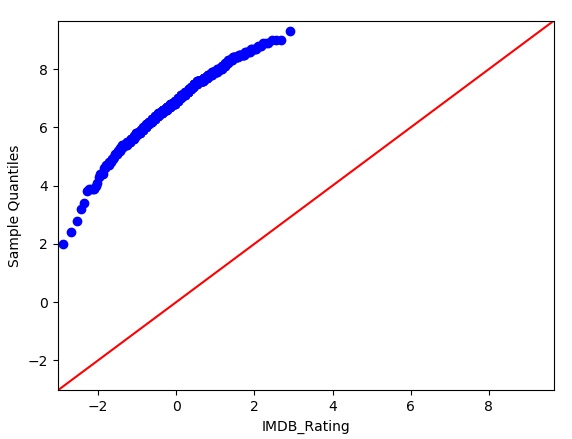
\includegraphics[scale=1.0]{graph_5}
 \caption{Q-Q діаграмма для  "IMDb рейтингу"} 
\end{figure}

Точки на графіку будують не-лінійний паттерн, отже розподіл цієї вибірки не є нормальним.

\Section{Висновки}

Виконуючи цю лабораторну роботу я навчився зчитувати .csv файли, будувати графіки і діаграми з отриманих даних, а також аналізувати їх.

\end{document}
